% !Rnw weave = knitr
% !TeX program = pdflatex

\documentclass[11pt]{article}\usepackage[]{graphicx}\usepackage[dvipsnames]{xcolor}
% maxwidth is the original width if it is less than linewidth
% otherwise use linewidth (to make sure the graphics do not exceed the margin)
\makeatletter
\def\maxwidth{ %
  \ifdim\Gin@nat@width>\linewidth
    \linewidth
  \else
    \Gin@nat@width
  \fi
}
\makeatother

\definecolor{fgcolor}{rgb}{0.345, 0.345, 0.345}
\newcommand{\hlnum}[1]{\textcolor[rgb]{0.686,0.059,0.569}{#1}}%
\newcommand{\hlsng}[1]{\textcolor[rgb]{0.192,0.494,0.8}{#1}}%
\newcommand{\hlcom}[1]{\textcolor[rgb]{0.678,0.584,0.686}{\textit{#1}}}%
\newcommand{\hlopt}[1]{\textcolor[rgb]{0,0,0}{#1}}%
\newcommand{\hldef}[1]{\textcolor[rgb]{0.345,0.345,0.345}{#1}}%
\newcommand{\hlkwa}[1]{\textcolor[rgb]{0.161,0.373,0.58}{\textbf{#1}}}%
\newcommand{\hlkwb}[1]{\textcolor[rgb]{0.69,0.353,0.396}{#1}}%
\newcommand{\hlkwc}[1]{\textcolor[rgb]{0.333,0.667,0.333}{#1}}%
\newcommand{\hlkwd}[1]{\textcolor[rgb]{0.737,0.353,0.396}{\textbf{#1}}}%
\let\hlipl\hlkwb

\usepackage{framed}
\makeatletter
\newenvironment{kframe}{%
 \def\at@end@of@kframe{}%
 \ifinner\ifhmode%
  \def\at@end@of@kframe{\end{minipage}}%
  \begin{minipage}{\columnwidth}%
 \fi\fi%
 \def\FrameCommand##1{\hskip\@totalleftmargin \hskip-\fboxsep
 \colorbox{shadecolor}{##1}\hskip-\fboxsep
     % There is no \\@totalrightmargin, so:
     \hskip-\linewidth \hskip-\@totalleftmargin \hskip\columnwidth}%
 \MakeFramed {\advance\hsize-\width
   \@totalleftmargin\z@ \linewidth\hsize
   \@setminipage}}%
 {\par\unskip\endMakeFramed%
 \at@end@of@kframe}
\makeatother

\definecolor{shadecolor}{rgb}{.97, .97, .97}
\definecolor{messagecolor}{rgb}{0, 0, 0}
\definecolor{warningcolor}{rgb}{1, 0, 1}
\definecolor{errorcolor}{rgb}{1, 0, 0}
\newenvironment{knitrout}{}{} % an empty environment to be redefined in TeX

\usepackage{alltt}

\usepackage[margin=1in]{geometry}
\usepackage[T1]{fontenc}
\usepackage[utf8]{inputenc}
\usepackage[american]{babel}
\usepackage{lmodern}
\usepackage{microtype}
\usepackage{authblk}
\usepackage[dvipsnames]{xcolor}
\usepackage{amsmath,amssymb,mathtools}
\usepackage{booktabs,threeparttable,tabularx,array}
\usepackage{caption}
\usepackage{float}
\usepackage{placeins}
\usepackage{todonotes}

\usepackage[most]{tcolorbox}

\newtcolorbox{plainlanguagebox}{
  breakable,
  colback=DemBlue!6,
  colframe=DemBlue!70!black,
  coltitle=white,
  fonttitle=\bfseries,
  title={In simple terms},
  boxrule=0.8pt,
  arc=2mm,
  left=8pt,
  right=8pt,
  top=7pt,
  bottom=7pt
}

\usepackage{tikz}
\usetikzlibrary{positioning,arrows.meta,fit,calc}
\usepackage{csquotes}
\usepackage[hidelinks]{hyperref}
\usepackage[capitalize,noabbrev]{cleveref}
\usepackage[
  backend=biber,
  style=authoryear,
  dashed=false,
  doi=false,
  isbn=false,
  url=false,
  arxiv=false,
  uniquename=false,
  uniquelist=false
]{biblatex}
\addbibresource{references.bib}
\addbibresource{/Users/hectorbahamonde/Bibliografia_PoliSci/library.bib}
\addbibresource{/Users/hectorbahamonde/research/reslide/references.bib}
\addbibresource{/Users/hectorbahamonde/Bibliografia_PoliSci/Bahamonde_BibTex2013.bib}

\definecolor{DemBlue}{HTML}{264653}
\definecolor{ExecOrange}{HTML}{E76F51}
\definecolor{RecoveryGreen}{HTML}{2A9D8F}
\definecolor{LightBlue}{HTML}{EAF2F4}
\definecolor{LightOrange}{HTML}{FBEDE9}
\definecolor{PersistPurple}{HTML}{6D597A}
\newcommand{\Dproc}{\textsf{D}}
\newcommand{\Aproc}{\textsf{A}}
\newcommand{\ind}[1]{\mathbb{1}\{#1\}}

\title{\textbf{\input{title.txt}\unskip}}
\author[1,2]{\textsc{Hector Bahamonde}\thanks{\href{mailto:hector.bahamonde@utu.fi}{hector.bahamonde@utu.fi}; \href{https://www.hectorbahamonde.com}{\texttt{hectorbahamonde.com}}}}
\affil[1]{INVEST Research Flagship Centre, University of Turku, Finland}
\affil[2]{Social Science Research Institute, \AA bo Akademi University, Finland}
\date{Working proposal --- \today}
\IfFileExists{upquote.sty}{\usepackage{upquote}}{}
\begin{document}
\pagenumbering{gobble}
\maketitle

\begin{abstract}
Why do citizens who accept weakly constrained leadership under adverse conditions return to collective control when those conditions improve? I study \emph{undemocratic reversal}: a within-person shift from authorizing leader discretion back to a citizen-controlled procedure after the structural justification for discretion disappears. The project uses a one-session, incentivized laboratory experiment with two consecutive ten-round blocks. In every round, five participants vote between a citizen-led and a leader-led method for funding public services. The leader-led method can produce services more effectively, but one participant controls the group decision and may move public-service points to a personal account. Block 1 gives that method a productive advantage. Before Block 2, ten-person matching pools are randomly assigned either to recovery, which removes the advantage, or to persistence, which retains it. The design observes two distinct aspects of democratic backsliding: participants may \emph{authorize} weak constraints by voting for the leader-led method, and selected leaders may \emph{use} that discretion by appropriating shared resources. The primary outcome is whether a participant who supported leader control at the end of Block 1 returns to citizen control at the end of Block 2. All twenty ballots, leader decisions, public-service allocations, and realized payoffs trace this reversal within a single synchronized session. \\ {\vspace{5cm}\color{red}See prototype here}: \url{https://panel-lab-experiment.onrender.com}
\end{abstract}


\clearpage
\pagenumbering{arabic}
\setcounter{page}{1}

\section{Research Question and Contribution}

Democratic backsliding research has established that citizens can learn to tolerate norm violations when structural threats make such tolerance instrumentally attractive. The focus of this proposal is whether that learning is reversible when those structural conditions improve. Thus, the most intriguing finding in recent democratic backsliding research is not that citizens tolerate norm violations \parencite{GRAHAM2020}. My claim is that they \textit{learn} to do so. As citizens secularly experience norm-violating leaders and accumulate information about non-democratic behaviors \parencite{Levitsky:2018aa}, they recalibrate expectations, adjust their definitions of democracy itself \parencite{Ananda2021}, and gradually become ``normalized'' to authoritarianism \parencite{78328}. Yet this learning process raises a critical question: \textbf{Can that undemocratic learning be reversed?} If citizens can learn authoritarian tolerance, can they \emph{un}-learn it when the institutional conditions and threats that gave rise to such undemocratic leaders change? And critically, which institutional conditions trigger such reversals? These questions are fundamental for democratic resilience, and importantly, for \emph{defending} democracy \parencite{Capoccia2007a}.

This proposal asks:

\begin{quote}
\emph{When the structural conditions that made executive discretion instrumentally attractive improve, do citizens return to constrained collective government, and through what learning and memory processes?}
\end{quote}

Thus, this study focuses on this behavioral transition in the context of \emph{undemocratic reversal}. It is not simply low support for an undemocratic alternative, nor a between-person difference in democratic attitudes. It is an observed within-person change: a participant initially endorses an institution that concentrates authority and weakens ex ante control, then later chooses an institution that restores collective choice and constraints. The concept therefore requires a panel structure and at least two consequential institutional choices by the same person.

The design contributes to the literature in three ways. First, it turns democratic constraint into a set of payoff-relevant rules governing interaction. Participants do not merely rate political descriptions (vignettes). Their ballots select who controls endowments, how a public good is produced, and whether an executive may extract a private rent. This embeds democratic trade-offs in the public-good provision, delegation and voting literatures \parencite{Hamman2011}.

Second, it identifies a structural cause of reversal. All participants encounter low institutional capacity in Wave 1: ``{\bf Imagine that you are a citizen in a society where public services have been under serious strain for a long time. Parliament has failed to pass a budget for eight months, healthcare waiting times have doubled, and planning for public services has stalled.}.'' For Wave 2, matched pools are randomly assigned either to recovered capacity or to persistent incapacity. The executive institution itself does not improve or deteriorate. Consequently, the treatment changes the instrumental case for delegation rather than supplying a moral appeal to democracy.

Third, the experiment observes the mechanism rather than only its endpoint. Participants report what they remember after a one-week delay, state their expectation that institutional capacity recovered, vote in every round, and experience endogenous decisions by other subjects. The resulting record distinguishes durable learning from strategic adaptation and repeated-game dynamics.

\section{Theory}

\subsection{Conditional tolerance of unconstrained authority}

Citizens need not reject democratic constraints in principle to support an unconstrained executive in practice. They may instead accept discretion conditionally, i.e., when institutions appear incapable of producing valued outcomes. This logic is compatible with evidence that electoral and material considerations can outweigh checks on executives and that citizens interpret democratic violations through partisan and performance-based trade-offs \parencite{7f36f,0b3bf,33fbf}. It also clarifies why democratic tolerance can be learned: repeated evidence of institutional failure changes the expected payoff from retaining constraints.

In the experiment, the citizen-led procedure (\Dproc) preserves individual control: each person decides how many points to place in a public-services fund, and no one can remove points from that fund for personal use. Its low Block-1 productivity, however, makes public-service provision difficult. The leader-led procedure (\Aproc) represents a faster coordinated response: one person makes the decision for all five citizens, and the remaining fund is converted into public services more effectively. The same leader may also move part of the fund to a personal account. The productive multiplier gives the speed-and-capacity advantage a consequential payoff counterpart rather than relying only on a vignette claim. A participant can therefore support \Aproc{} without expressing a general taste for autocracy. Under weak institutional capacity, concentrating authority can be an instrumentally attractive response to poor performance.

\paragraph{H1: Crisis endorsement.} In Block 1, support for the leader-led method will increase when participants' experience indicates that its productive advantage outweighs the risk of personal appropriation.

\subsection{Authorization and enactment of backsliding}

Democratic backsliding involves more than the presence of a self-interested leader. It also depends on whether citizens authorize arrangements that weaken collective control and on what officeholders do with the discretion they receive. The experiment separates these behavioral margins. A ballot for \Aproc{} authorizes one participant to decide for everyone, weakens ex ante control over the group's resources, and accepts the possibility of personal appropriation. Conditional on being selected as leader, the transfer $\rho$ records whether and how extensively that participant uses the granted discretion for personal gain.

This distinction connects the public-good game to democratic backsliding without treating a stylized allocation as literal corruption. Voting for \Aproc{} is an \emph{enabling} act; moving public-service points to a personal account is an \emph{enactment} of the distributive risk that weakened constraints create. Subsequent ballots then show how participants respond to both institutional performance and observed misuse. The design can therefore study individual adherence to collective control in a transparent incentive environment, rather than asking respondents whether appropriation is likely in contemporary Finland.

\paragraph{H2: Use of discretion.} Some selected leaders will move public-service points to their personal accounts, and larger observed transfers will be followed by lower support for the leader-led method among exposed participants.

\subsection{Structural updating and democratic reversal}

The central theoretical claim is conditional. If support for leader discretion was learned from weak structural performance, then credible improvement should reverse it. Before Block 2, recovery raises the citizen-led method's productivity to the leader-led method's level. Recovery therefore removes the leader's technological advantage while leaving the leader's discretion to appropriate points unchanged. Once citizens can produce public services equally well without surrendering control, the instrumental case for delegation disappears.

The persistence condition supplies the counterfactual. All participants remain in the same session, receive a Block-2 description, and play the same number of additional rounds; only the productivity of the citizen-led method differs. The treatment contrast therefore separates recovery-induced reversal from additional experience, fatigue, end-game behavior, and regression to the mean. The design identifies structural updating and within-session reversal with no return-visit attrition.

\paragraph{H3: Structural updating.} Participants assigned to recovery will report a larger increase in perceived citizen-led capacity and a larger reduction in the perceived need for leader control than participants assigned to persistence.

\paragraph{H4: Democratic reversal.} Among participants who choose \Aproc{} in Block 1's final round, assignment to recovery will increase the probability of choosing \Dproc{} in Block 2's final round.

\paragraph{H5: Behavioral path.} Recovery will change the path of institutional choice across Block 2: support for \Dproc{} should rise once its restored productivity is disclosed, while exposure to leader appropriation should make continued delegation less attractive.

\section{Experimental Design}

\subsection{Overview}

The study consists of one synchronized laboratory session lasting approximately 75--90 minutes. Participants complete two consecutive ten-round blocks and remain in stable ten-person matching pools throughout. Before each paid round, the software anonymously divides every pool into two temporary five-person groups. The Block-2 condition is randomized at the pool level and disclosed between blocks. Participants therefore interact repeatedly within a treatment-consistent local population but cannot build a reliable bilateral reputation.

\begin{figure}[H]
\centering
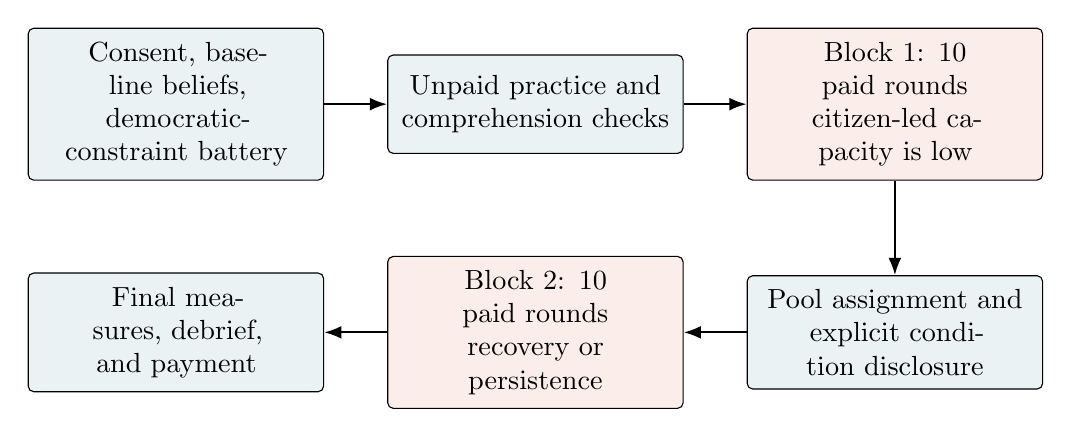
\begin{tikzpicture}[
  node distance=8mm and 8mm,
  box/.style={draw,rounded corners=2pt,align=center,text width=3.4cm,minimum height=1.25cm,inner sep=5pt},
  arr/.style={-{Latex[length=2.2mm]},thick}
]
\node[box,fill=LightBlue] (base) {Consent, baseline beliefs,\\democratic-constraint battery};
\node[box,fill=LightBlue,right=of base] (w1info) {Unpaid practice and\\comprehension checks};
\node[box,fill=LightOrange,right=of w1info] (w1game) {Block 1: 10 paid rounds\\citizen-led capacity is low};
\node[box,fill=LightBlue,below=12mm of w1game] (random) {Pool assignment and\\explicit condition disclosure};
\node[box,fill=LightOrange,left=of random] (w2game) {Block 2: 10 paid rounds\\recovery or persistence};
\node[box,fill=LightBlue,left=of w2game] (finish) {Final measures, debrief,\\and payment};
\draw[arr] (base) -- (w1info);
\draw[arr] (w1info) -- (w1game);
\draw[arr] (w1game) -- (random);
\draw[arr] (random) -- (w2game);
\draw[arr] (w2game) -- (finish);
\end{tikzpicture}
\caption{One-session experimental sequence. Every paid round contains a secret institutional ballot, an institution-contingent allocation decision, feedback, and anonymous rematching.}
\label{fig:design}
\end{figure}

\begin{figure}[H]
\centering
\resizebox{\linewidth}{!}{%
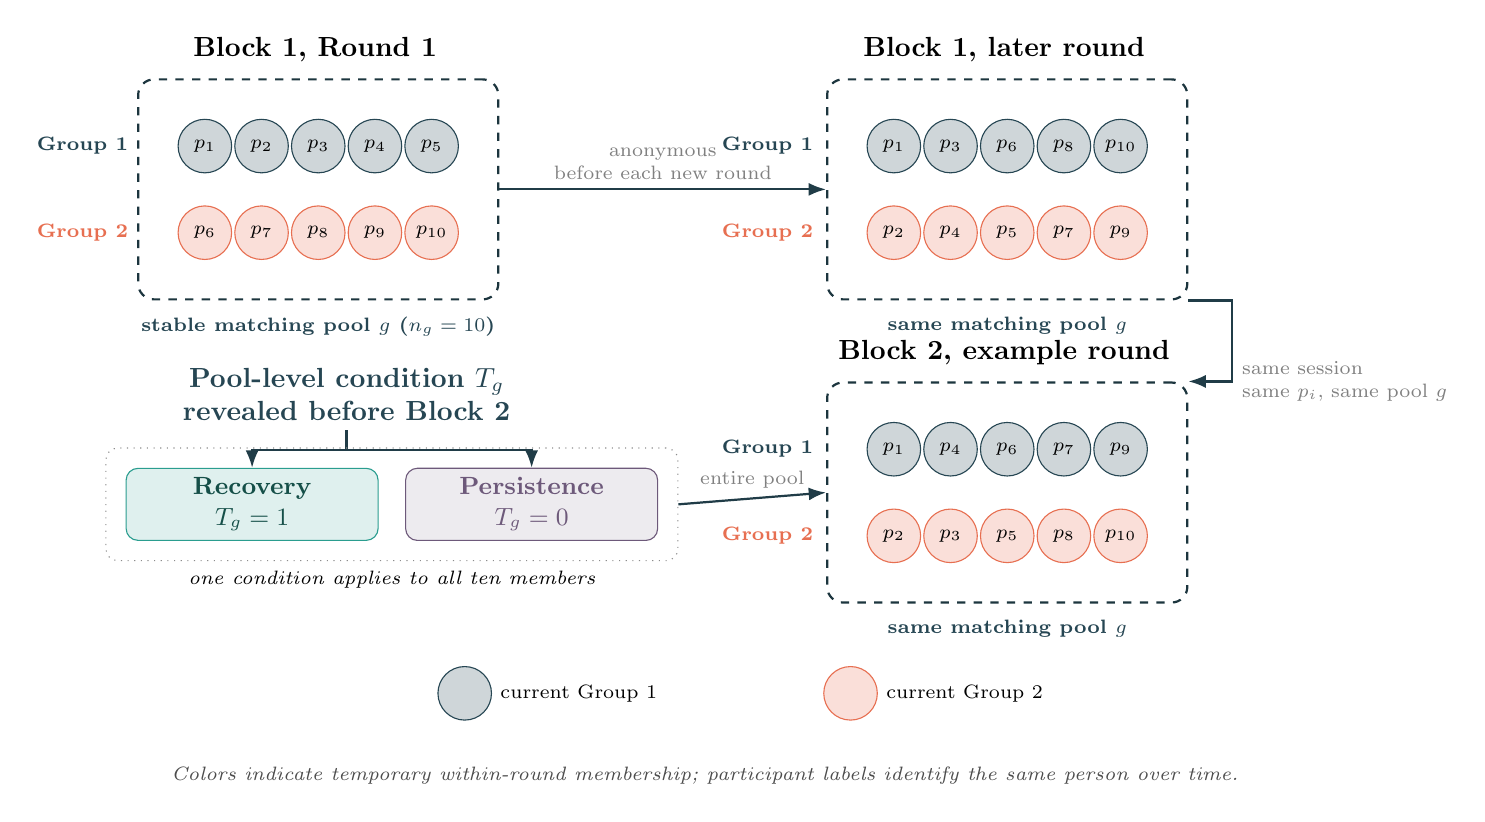
\begin{tikzpicture}[
  font=\small,
  >=Latex,
  person/.style={circle,draw,minimum size=6.8mm,inner sep=0pt,font=\scriptsize\bfseries},
  groupone/.style={person,draw=DemBlue,fill=DemBlue!22},
  grouptwo/.style={person,draw=ExecOrange,fill=ExecOrange!22},
  poolbox/.style={draw=DemBlue!75!black,dashed,rounded corners=2mm,line width=0.8pt,inner sep=5mm},
  treatment/.style={draw,rounded corners=1.5mm,align=center,minimum width=3.2cm,minimum height=8mm,font=\small\bfseries},
  flow/.style={-{Latex[length=2.2mm]},line width=0.8pt,draw=DemBlue!85!black},
  groupname/.style={font=\scriptsize\bfseries,anchor=east},
  snapshot/.style={font=\bfseries,anchor=south}
]

% Block 1, Round 1
\node[snapshot] at (2.25,3.95) {Block 1, Round 1};
\node[groupname,text=DemBlue] at (0,3.00) {Group 1};
\foreach \lab [count=\k from 0] in {1,2,3,4,5} {
  \node[groupone] (wonea\lab) at ({0.85+0.72*\k},3.00) {$p_{\lab}$};
}
\node[groupname,text=ExecOrange] at (0,1.90) {Group 2};
\foreach \lab [count=\k from 0] in {6,7,8,9,10} {
  \node[grouptwo] (woneb\lab) at ({0.85+0.72*\k},1.90) {$p_{\lab}$};
}
\node[poolbox,fit=(wonea1)(wonea5)(woneb6)(woneb10)] (poolone) {};
\node[font=\scriptsize\bfseries,text=DemBlue,anchor=north]
  at ($(poolone.south)+(0,-0.08)$) {stable matching pool $g$ ($n_g=10$)};

% Block 1, later round after rematching
\node[snapshot] at (11.00,3.95) {Block 1, later round};
\node[groupname,text=DemBlue] at (8.7,3.00) {Group 1};
\foreach \lab [count=\k from 0] in {1,3,6,8,10} {
  \node[groupone] (wonera\lab) at ({9.60+0.72*\k},3.00) {$p_{\lab}$};
}
\node[groupname,text=ExecOrange] at (8.7,1.90) {Group 2};
\foreach \lab [count=\k from 0] in {2,4,5,7,9} {
  \node[grouptwo] (wonerb\lab) at ({9.60+0.72*\k},1.90) {$p_{\lab}$};
}
\node[poolbox,fit=(wonera1)(wonera10)(wonerb2)(wonerb9)] (poollater) {};
\node[font=\scriptsize\bfseries,text=DemBlue,anchor=north]
  at ($(poollater.south)+(0,-0.08)$) {same matching pool $g$};

\draw[flow] (poolone.east) -- node[above,align=center,font=\scriptsize]{{\color{gray}anonymous}\\{\color{gray}before each new round}} (poollater.west);

% Pool-level condition for Block 2
\node[align=center,font=\bfseries,text=DemBlue] (assignment) at (2.65,-0.15)
  {Pool-level condition $T_g$\\revealed before Block 2};
\node[treatment,draw=RecoveryGreen,fill=RecoveryGreen!15,text=RecoveryGreen!50!black]
  (recovery) at (1.45,-1.55) {Recovery\\$T_g=1$};
\node[treatment,draw=PersistPurple,fill=PersistPurple!12,text=PersistPurple]
  (persistence) at (5.00,-1.55) {Persistence\\$T_g=0$};
\draw[flow] (assignment.south) -- ++(0,-0.25) -| (recovery.north);
\draw[flow] (assignment.south) -- ++(0,-0.25) -| (persistence.north);
\node[draw=black!45,dotted,rounded corners=1.5mm,fit=(recovery)(persistence),inner sep=2.5mm,
      label={[font=\scriptsize\itshape,align=center]below:one condition applies to all ten members}]
  (conditionbox) {};

% Block 2: same participants, same pool, new temporary groups
\node[snapshot] at (11.00,0.10) {Block 2, example round};
\node[groupname,text=DemBlue] at (8.7,-0.85) {Group 1};
\foreach \lab [count=\k from 0] in {1,4,6,7,9} {
  \node[groupone] (wtwoa\lab) at ({9.60+0.72*\k},-0.85) {$p_{\lab}$};
}
\node[groupname,text=ExecOrange] at (8.7,-1.95) {Group 2};
\foreach \lab [count=\k from 0] in {2,3,5,8,10} {
  \node[grouptwo] (wtwob\lab) at ({9.60+0.72*\k},-1.95) {$p_{\lab}$};
}
\node[poolbox,fit=(wtwoa1)(wtwoa9)(wtwob2)(wtwob10)] (pooltwo) {};
\node[font=\scriptsize\bfseries,text=DemBlue,anchor=north]
  at ($(pooltwo.south)+(0,-0.08)$) {same matching pool $g$};

\draw[flow] (poollater.south east) -- ++(0.55,0) |-
  node[pos=0.50,right,align=left,font=\scriptsize]{{\color{gray}same session}\\{\color{gray}same $p_i$, same pool $g$}}
  (pooltwo.north east);
\draw[flow] (conditionbox.east) -- node[above,font=\scriptsize]{{\color{gray}entire pool}} (pooltwo.west);

% Legend
\node[groupone] at (4.15,-3.95) {};
\node[anchor=west,font=\scriptsize] at (4.48,-3.95) {current Group 1};
\node[grouptwo] at (9.05,-3.95) {};
\node[anchor=west,font=\scriptsize] at (9.38,-3.95) {current Group 2};
\node[font=\scriptsize\itshape,align=center,text=black!70] at (7.20,-5)
  {Colors indicate temporary within-round membership; participant labels identify the same person over time.};

\end{tikzpicture}%
}
\caption{Matching pools, anonymous rematching, and Block-2 treatment assignment.}
\label{fig:pool-rematching}
\end{figure}


\begin{plainlanguagebox}
The design uses permanent ten-person matching pools, denoted by $g$. Before each paid round, the software divides every pool into two temporary five-person groups that vote and play separately. These groups dissolve after the round and are formed again before the next one. Participants never interact outside their pool. Accordingly, the colors in \cref{fig:pool-rematching} show current-round group membership, while $p_i$ identifies the same participant throughout the session. Before Block 2, the entire pool learns that citizen-led public-service capacity has either recovered ($T_g=1$) or remains under strain ($T_g=0$). The planned sample repeats this structure across 40 pools.

This arrangement creates interaction without fixed teams. Its principal cost is repeated exposure within pools, but anonymity and rematching limit partner-specific reputation, collusion, and retaliation while preserving social learning. Stable pools also keep potential spillovers within treatment-homogeneous environments, provide 40 independently randomized clusters, and permit two complete five-person groups in every round.

Statistically, democratic reversal ($R_i$) is measured for each participant $p_i$, whereas treatment ($T_g$) is assigned to the pool. Individual outcomes are therefore compared across treatment conditions with standard errors clustered by pool. The temporary five-person groups organize play but are not independent treatment units.
\end{plainlanguagebox}

%The ten rounds per block permit participants to experience both methods, observe leader choices, and reveal whether reversal is immediate, gradual, or unstable. The primary endpoint remains the final ballot in each block; earlier rounds process-trace the trajectory and do not multiply the number of independent treatment units.

\subsection{The institutional-choice public-good game}

Each round begins with 20 points for each of five group members. Every member privately votes between the citizen-led procedure (\Dproc) and the leader-led procedure (\Aproc). A simple majority of at least three votes selects the binding method. Individual ballots remain secret; the group sees the aggregate vote and the selected rule. The neutral labels shown to participants are ``Citizens decide'' and ``A leader decides.''

\paragraph{Citizen-led procedure (\Dproc).} Each member chooses an allocation $c_i$ of 0--20 points to a public-services fund; unallocated points remain in the member's personal account. Let $m_{gb}$ denote the fund's productivity for matching pool $g$ in block $b$. Player $i$ earns
\begin{equation}
\pi^{D}_{igbr}=20-c_{igbr}+\frac{m_{gb}}{5}\sum_{j=1}^{5}c_{jgbr}.
\label{eq:democratic}
\end{equation}
The marginal private return is below 1 in both capacity states, preserving the social dilemma, while the group return exceeds 1. In Block 1, $m_{g1}=1.50$ for everyone. In Block 2, $m_{g2}=2.50$ under recovery and $m_{g2}=1.50$ under persistence.

\paragraph{Leader-led procedure (\Aproc).} One group member is selected as leader. Selection is balanced toward members who have served least often, with random resolution of ties. The leader chooses the number of points $t\in\{0,\ldots,20\}$ that every citizen must place in the public-services fund. The leader may then move $\rho\in\{0,\ldots,20\}$ fund points to a personal account, subject to $\rho\leq 5t$. The remaining fund $5t-\rho$ always uses multiplier 2.50. A nonleader earns
\begin{equation}
\pi^{A}_{igbr}=20-t+\frac{2.50}{5}(5t-\rho),
\label{eq:executive-nonleader}
\end{equation}
while the leader earns
\begin{equation}
\pi^{A,L}_{igbr}=20-t+\frac{2.50}{5}(5t-\rho)+\rho.
\label{eq:executive-leader}
\end{equation}
All members observe the required allocation, the amount moved to the leader's personal account, the public-service return, and their own payoff. Leader control can coordinate provision and, in Block 1, produces public services more effectively. It also creates a distributive conflict grounded in another participant's decision.


\begin{plainlanguagebox}
Each round starts with 20 points for each citizen. The five citizens first cast private ballots ($V_{ibr}\in\{\Dproc,\Aproc\}$) about who should make the public-service decision. If at least three vote for ``Citizens decide'' ($\Dproc$), each citizen chooses how many points to put in the public-services fund ($c_{igbr}$). The software adds those points, multiplies the fund by the current rate ($m_{gb}$), and divides the result equally among all five citizens. Points not put in the fund remain in each citizen's personal account.

If at least three vote for ``A leader decides'' ($\Aproc$), the software appoints one group member, randomly selecting among those who have served least often. Participants therefore choose the decision method, not a particular candidate; there is no campaign. The leader decides how many points every citizen must put in the fund ($t$). The leader may then move up to 20 of those fund points to a personal account ($\rho\leq\min\{20,5t\}$). The points left in the fund ($5t-\rho$) are multiplied by 2.50 and divided equally among all five citizens; the leader also keeps the amount moved.

At the end of the round, everyone sees the selected method, the fund decisions, any amount moved by the leader, the public-service return, and their own payoff ($\pi^{D}_{igbr}$ under \Dproc{} or $\pi^{A}_{igbr}$ under \Aproc{}). The temporary group then dissolves, and participants are anonymously rematched within their ten-person pool ($g$).
\end{plainlanguagebox}


\begin{table}[H]
\centering
\caption{Implemented design parameters}
\label{tab:parameters}
\begin{threeparttable}
\begin{tabularx}{\textwidth}{>{\raggedright\arraybackslash}p{0.29\textwidth} X}
\toprule
Feature & Implemented value \\
\midrule
Laboratory session & One synchronized visit, approximately 75--90 minutes \\
Paid rounds & 10 per block (20 total), preceded by unpaid practice \\
Group and matching pool & 5-person groups; 10-person treatment-matched pools \\
Rematching & Anonymous rematching within pool before every paid round \\
Round endowment & 20 points per participant \\
Citizen-led multiplier & 1.50 in Block 1; 2.50 recovery / 1.50 persistence in Block 2 \\
Leader-led multiplier & 2.50 in both blocks and conditions \\
Leader's personal transfer & 0--20 fund points, limited by the number of points in the fund \\
Performance payment & One randomly selected game round from each block \\
Exchange rate & EUR 0.20 per point \\
Show-up payment & EUR 10.00 \\
\bottomrule
\end{tabularx}
\begin{tablenotes}[flushleft]\footnotesize
\item The random-round rule limits wealth effects, hedging across rounds, and excessive payment while preserving incentives in every decision.
\end{tablenotes}
\end{threeparttable}
\end{table}

\subsection{Block 1: crisis and leader authorization}

After consent, participants receive common instructions, complete baseline capacity and risk beliefs, and answer a seven-item democratic-constraint battery. They then complete an unpaid guided practice covering citizen and leader decisions, the ballot, and random-round payment. Three comprehension questions must be answered correctly before production play begins; responses are optional in the development configurations. The Block-1 instructions describe a hypothetical society in a prolonged public-service crisis. When citizens decide individually, each point left in the fund produces 1.50 points for the group. When a leader decides, each point left in the fund produces 2.50 points, but the leader may move as many as 20 fund points to a personal account.

Participants then play ten paid rounds. Every round follows the same sequence: secret institutional ballot; majority rule; fund decisions under \Dproc{} or leader decisions under \Aproc; simultaneous feedback; and rematching. After Round 10, capacity and risk beliefs and the constraint battery are measured again. The software records the final ballot, leader support in Rounds 8--10, all fund decisions, all personal transfers, and realized payoffs. One Block-1 round is randomly chosen for payment.

\subsection{Block 2: structural change and reversal}

Immediately after Block 1, each ten-person pool is assigned to one of two environments. Under \emph{recovery}, the citizen-led multiplier rises from 1.50 to 2.50. Under \emph{persistence}, it remains 1.50. The leader-led multiplier, authority, and maximum personal transfer remain fixed. A transition page explicitly states the rates that apply in Block 2. Participants do not have to infer a hidden state: the treatment is a transparent change in the relative institutional trade-off.

Participants then play ten additional rounds. The same ballot, leader rule, group size, and payoff sequence make behavior directly comparable across blocks. After Round 10, the capacity and risk measures and constraint battery are repeated. The final Block-2 ballot is the reversal endpoint. One Block-2 round is randomly paid; the two selected-round payoffs are converted to euros and added to the participation payment.

\section{Learning Across Repeated Play: Design Safeguards}

Repeated play is an advantage only if procedural learning is not confused with the substantive learning of interest. The design therefore anticipates six implementation concerns.

\paragraph{Procedural learning.} Participants may initially misunderstand payoff rules and improve merely through practice. A guided unpaid block and mandatory comprehension checks move rule learning before the paid data. Round 1 remains available for diagnostics, while the preregistered endpoint uses Round 10 and the late-round mean uses Rounds 8--10.

\paragraph{Reputation and reciprocity.} Fixed five-person groups would allow personal histories to drive votes and contributions. Anonymous rematching within ten-person pools breaks stable bilateral relationships while keeping treatment exposure and synchronized interaction feasible. Participants never receive persistent identities.

\paragraph{Leader-role learning.} Subjects could support delegation because they expect to become leader. Assignment is balanced among the least-served eligible members, preventing a few participants from monopolizing the role. Analyses will nevertheless describe prior leader service and realized personal transfers.

\paragraph{Endogenous institutional experience.} Groups that never elect one procedure receive less experience with it. Instructions and practice expose everyone to both payoff rules, and realized experience is recorded. Treatment effects will be reported by prior exposure, but the primary intention-to-treat contrast will not condition on a post-treatment institutional path.

\paragraph{Wealth, fatigue, and end-game effects.} Only one randomly selected round per block determines game earnings, so earnings from early rounds do not alter later endowments. Instructions explain that every round has an equal payment chance. The ten-round horizon is disclosed and identical across conditions. Page timers, decision times, and timeouts identify fatigue or end-game behavior. The persistence group experiences the same twenty-round sequence as the recovery group, separating the treatment effect from generic within-session fatigue.

\paragraph{Cross-block comparability.} The method labels, leader rules, endowments, sequence, pool structure, and number of rounds are held constant. Recovery changes only the citizen-led fund multiplier. The persistence group identifies change caused by additional play, repeated measurement, or approaching the end of the session.

These safeguards do not attempt to eliminate all learning. The study requires participants to learn from consequences. They instead separate theoretically meaningful learning about institutional performance from avoidable learning about the interface or accidental partners.

\section{Outcomes, Process Measures, and Estimands}

Let $V_{ibr}\in\{\Dproc,\Aproc\}$ be participant $i$'s ballot in block $b$ and round $r$. Define Block-1 leader endorsement as
\begin{equation}
A_{i1}=\ind{V_{i,1,10}=\Aproc}.
\end{equation}
For the theoretically relevant subgroup with $A_{i1}=1$, democratic reversal is
\begin{equation}
R_i=\ind{V_{i,2,10}=\Dproc}.
\end{equation}
Let $T_g=1$ indicate that matching pool $g$ received structural institutional recovery. The primary causal estimand is
\begin{equation}
\tau_R=\mathbb{E}[R_i(1)-R_i(0)\mid A_{i1}=1],
\end{equation}
estimated as an intention-to-treat contrast with standard errors clustered by the ten-person randomization pool. Because $A_{i1}$ is measured in Block 1, before the Block-2 condition is disclosed, defining this subgroup does not condition on a post-treatment variable. The primary model will include prespecified baseline covariates only for precision; an unadjusted difference in means will also be reported.

\begin{plainlanguagebox}
The primary causal estimand ($\tau_R$) asks: among participants who chose ``A leader decides'' in the final round of Block 1 ($V_{i,1,10}=\Aproc$, summarized by $A_{i1}=1$), how much does assignment to recovery ($T_g=1$), rather than persistence ($T_g=0$), increase the probability that they return to ``Citizens decide'' in the final round of Block 2 ($V_{i,2,10}=\Dproc$), thereby constituting a democratic reversal ($R_i=1$)? Ideally, we would compare each participant's decision under recovery ($R_i(1)$) with the decision that the same participant would have made under persistence ($R_i(0)$). Because both outcomes cannot be observed for the same person, random assignment allows us to estimate this effect by comparing reversal rates between conditions. Participants are analyzed according to their pool's assigned condition ($T_g$), and statistical uncertainty is calculated at the pool level.
\end{plainlanguagebox}

The ballot measures authorization of leader discretion; the transfer $\rho_{igbr}$ measures its use. Define enacted appropriation among selected leaders as $M_{igbr}=\ind{\rho_{igbr}>0}$. Its intensity is recorded both in points and as a share of the available fund, $\rho_{igbr}/(5t_{igbr})$, when $t_{igbr}>0$. These outcomes are individual choices, but leader selection and prior institutional outcomes are endogenous. They are therefore treated as theoretically important behavioral and process measures rather than as randomized effects of recovery.

Three secondary ballot outcomes describe robustness: (1) the change in leader-vote share from Block-1 Rounds 8--10 to Block-2 Rounds 8--10; (2) the full round-by-treatment trajectory; and (3) group-level selection of each method. Fund allocations, required allocations, personal transfers, fund size, leader service, exposure to appropriation, and realized payoffs describe the strategic environment in which ballots change.

Process outcomes occur at baseline, after Block 1, and after Block 2. They include perceived public-service capacity, perceived risk to constraints, the seven-item constraint index, round-level ballots, fund decisions, leader decisions, and realized payoffs. Battery items are randomized once per participant and then stored, preventing re-randomization on refresh. Any decomposition through perceived capacity or exposure to leader behavior will be labeled exploratory unless supported by a preregistered causal mediation strategy. The clean confirmatory claim remains the pool-randomized effect of recovery on reversal.

\section{Randomization, Sample, and Power}

The planned sample is 400 participants organized into 40 ten-person matching pools. For administrative reproducibility, pools are assigned in approximately equal numbers to recovery and persistence when the session is created. Assignment changes no Block-1 parameter and is disclosed only at the transition to Block 2. Eliminating the return visit removes cross-visit attrition and broken panel links. Recruitment should nevertheless overbook each synchronized cohort and maintain a standby list because interaction requires complete five-person groups at the start of the session.

Power depends on three quantities that cannot responsibly be inferred from the twenty repeated decisions: the proportion endorsing \Aproc{} at the Block-1 endpoint, the persistence-group reversal rate, and the intrapool correlation. A pilot will estimate these values, after which power will be evaluated by simulation at the pool level under the planned assignment. Repeated rounds increase measurement reliability and identify trajectories; they do not turn 400 participants or 40 randomized pools into 8,000 independent observations.

Randomization code assigns whole ten-person pools and approximately balances the number of pools across conditions. Production sessions should contain a multiple of ten participants. If several laboratory rooms run concurrently, randomization and matching remain within the configured cohort so that participants never interact across inconsistent treatment states.

\section{Payments and Laboratory Operations}

At EUR 0.20 per point, the implemented parameters are designed to yield an expected total payment of roughly EUR 18--25, including the EUR 10 participation payment, depending on play. Final budgeting will use pilot distributions rather than theoretical maxima. At completion, the interface displays the selected Block-1 round, selected Block-2 round, point total, performance payment, participation payment, and total payment separately.

Both blocks are run during one synchronized session. The transition page is released only after every active participant has completed Block 1, so members of a matching pool encounter the new environment together. Participant codes, not names, link decisions across blocks, and all payments are made after Block 2.

The operational protocol requires complete groups. Standby participants may enter only before the first paid round. Once play begins, no replacement subject inherits another participant's history. Every strategic decision has a 90-second limit. If a participant times out, the software records the timeout and applies a neutral, prespecified default so that group members can continue. The session log must document late arrival, browser failure, early departure, manual intervention, and payment exceptions. Exclusion rules should be preregistered and should never depend on treatment-consistent behavior.

Before launch, two pilots are required. A technical pilot should use at least ten simultaneous clients and both treatment branches to stress wait pages, rematching, refresh persistence, timeouts, and payment calculations. A behavioral pilot should estimate duration, comprehension, Block-1 leader endorsement, leader appropriation, fatigue, and payoff distributions. Parameters should be frozen after that pilot and before confirmatory registration.

\section{Ethics and Interpretation}

The experiment exposes participants to a setting in which concentrated authority can be materially effective. That feature is necessary to study conditional tolerance, but it creates an obligation to avoid deception and moral labeling. Instructions therefore use the neutral labels ``Citizens decide'' and ``A leader decides,'' explain the public-services fund in plain language, and disclose exactly what the leader may do. The recovery condition is implemented through the programmed fund multiplier and explicitly announced before Block 2.

Consent explains the one-session structure, interaction, anonymity, payment rule, data linkage, and right to withdraw. The debrief explains the democratic interpretation only after all incentivized decisions and clarifies that no single vote or transfer establishes that a participant is corrupt, authoritarian, or opposed to democracy. Data exports should replace participant labels with study IDs and store the linkage key separately.

The Finnish setting strengthens the case for a hypothetical, incentive-based task. The experiment does not ask participants to judge whether Finnish officials appropriate public resources, nor does it present the scenario as a description of Finland. Instead, all participants face the same fictional public-service crisis and make consequential choices under transparent rules. Variation in their behavior therefore speaks to individual willingness to preserve collective control when concentrated authority offers material benefits, even in a population for whom public appropriation may otherwise seem remote.

The interpretation will remain narrow. Choosing the leader-led method in a stylized public-good environment is evidence about behavior under institutional trade-offs, not a complete measure of democratic commitment. The strongest contribution comes from the randomized change in those trade-offs and the observed within-person return to constraints.

\section{Planned Deliverables and Decision Rule}

The confirmatory package will contain the theory, hypotheses, full instructions, oTree code, randomization procedure, exclusion rules, primary estimand, and pool-level power simulation. The principal conclusion will follow a simple rule: evidence for structural democratic reversal requires a positive, substantively meaningful, and statistically distinguishable recovery effect on $R_i$ among Block-1 leader endorsers. Round-level trajectories, beliefs, fund decisions, leader choices, personal transfers, and allocations will be used to assess whether the observed endpoint follows the proposed learning mechanism and to identify rival explanations.

This design preserves the project's core ambition---observing people learn and then potentially unlearn tolerance for weakly constrained authority---while giving that learning a strategic and distributive foundation. Subjects vote over rules that govern other subjects, may personally exercise the discretion those rules create, experience the consequences, and choose again after an experimentally altered structure is disclosed in the same session.

\FloatBarrier
\printbibliography

\end{document}
